\section{\MC}
\label{sec:makecode}
% @TOM REVIEW:
The key technical contribution of \MC is to provide users with a safe environment to write programs for MCUs, enabling a simple progression from block-based
programming, to text-based programming in Static TypeScript (STS),
while leveraging C++ on the backend for efficient use of MCU resources.
Both C++ and TypeScript APIs can be specially annotated (minimally via
the \emph{//\% block} comment) so that the \MC compiler generates the required
Blocky metadata,
\MC uses the Blockly and Monaco editors to allow the user to code with
visual blocks or STS. The editing experience is parameterized by the full-typed device
runtime, which provides a set of categorized APIs to the end-user.

Figure~\ref{fig:screenSnap} shows a screen snapshot of the \MC web app for the Adafruit Circuit Playground Express (CPX), which has five sections:
(A) the menu bar allows switching between the two editors;
(B) the simulator shows the CPX board and provides feedback on user code executed in the browser;
(C) the toolbar provides access to device-specific APIs and programming elements;
(D) the programming canvas;
(E) the download button invokes the compiler to produce a binary executable.

The web app encapsulates all the components needed to deliver a programming experience
for MCUs, free of the need for a C++ compiler for the compilation of user code.
The web app is written in TypeScript and incorporates the TypeScript compiler and
language service as well.
The app is built from a \MC ``target''
which parameterizes the \MC framework for a particular device.
The remaining subsections describe the essential components of the web app
from Figure~\ref{fig:makecode}.


\begin{figure}[t]
    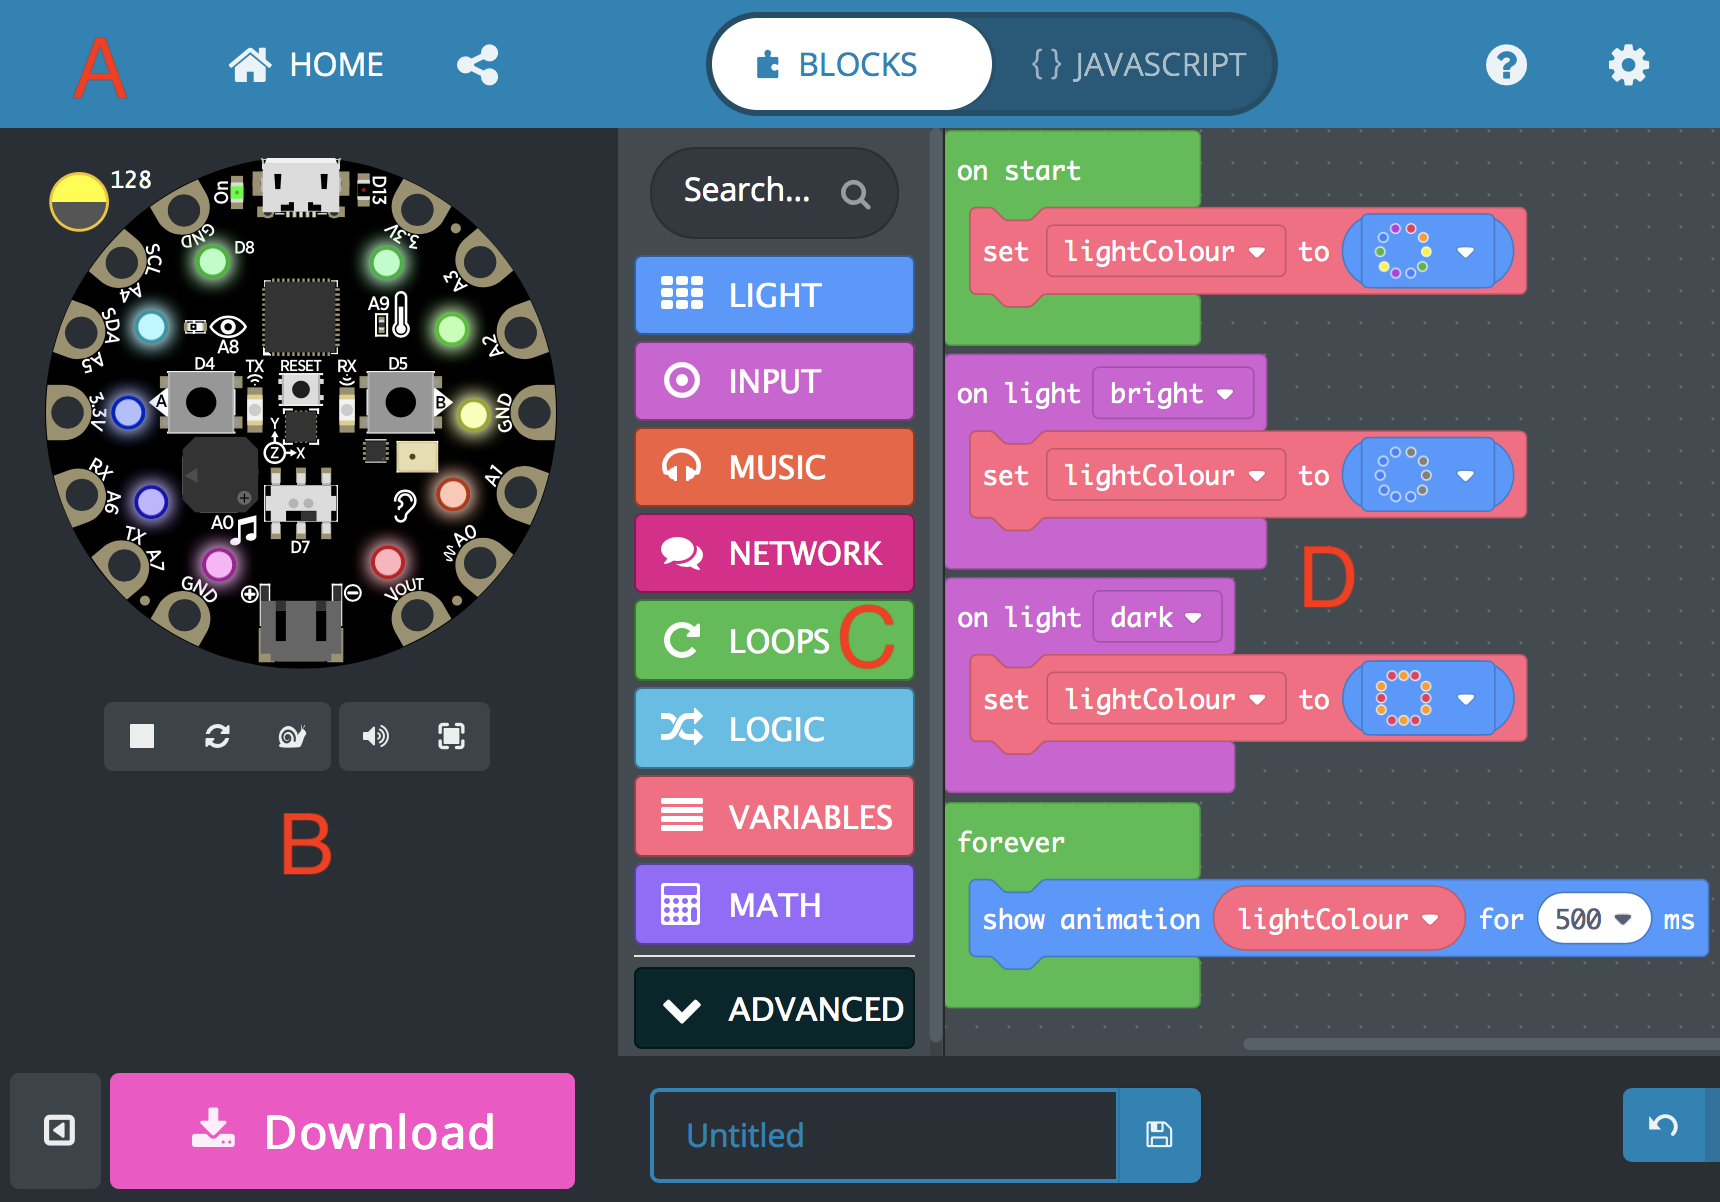
\includegraphics[width=\columnwidth]{images/CPXFig}
\caption{\label{fig:screenSnap}Screen snapshot of the \MC web app.}
\end{figure}

\subsection{Static TypeScript (STS)}

TypeScript is a typed superset of JavaScript designed to enable JavaScript developers to take advantage of code
completion, static checking and refactoring made possible by types (\url{http://www.typescriptlang.org/}).
As a starting point, every JavaScript program is a TypeScript program.  Types can be added gradually to such programs, supported by type inference. While TypeScript provides classes and interfaces with syntax like
Java/C\#, their semantics are quite different, as they are based on JavaScript. Classes are simply syntactic sugar for creating objects that have code associated with them, but these objects are
JavaScript objects with all their dynamic semantics intact

Static TypeScript is closely related to  StrongScript~\cite{StrongScriptECOOP15},
which extends TypeScript with a type constructor
for \emph{concrete} types, allowing the programmer to choose between untyped
code, optionally-typed code, and concretely typed code, which provides traditional
type soundness guarantees, as in Java and C\#.
STS can be seen to be StrongScript where every variable and
expression has a concrete type. As in StrongScript, classes are nominally typed,
which permits a more efficient and traditional property lookup for class instances.
STS goes further than StrongScript by outlawing downcasts.

\subsection{Device runtime and Shim Generation}
\label{sec:shim-gen}
A \MC target is defined, in part, by its device runtime, which is a combination of C++
and STS code, as shown in the lower-left of Figure~\ref{fig:makecode}.
All the target's C++ files are precompiled (by a C++ compiler in the cloud)
into a binary, which is stored in the cloud in a single blob, as well as in the HTML5 application cache. Additional runtime
components may be authored in STS, which allows the device runtime to be extended with or without the use of C++, and permits components of the device runtime to be shared by both the device
and simulator runtimes. The ability to author the device runtime in both STS and C++ is
a unique aspect of \MCN's design.

Whether runtime components are authored in C++ or STS, all runtime APIs are exposed as fully-typed
TypeScript definitions. A fully-typed runtime improves the end-user experience
by making it easier to discover APIs; it also enables the type inference provided by the TypeScript
compiler to infer types for (unannotated) user programs.

\MC supports a simple foreign function interface from STS to C++ based on namespaces,
enumerations, functions, and basic type mappings. \MC uses top-level namespaces to organize sets of related functions.  Preceding a C++ namespace, enumeration, or function
with a comment starting with \emph{//\%} indicates that \MC should map the C++ construct to STS.
Within the \emph{//\%} comment, attributes are used to define the visual appearance for that
language construct, such as for the input namespace in the C++ for the CPX:
\begin{lstlisting}
//% color="#B4009E" weight=98 icon="\uf192"
namespace input {
    ...
\end{lstlisting}

Figure~\ref{fig:screenSnap}(C) shows the toolbox of API and language categories, where the
category \emph{INPUT} corresponding to the namespace \emph{input} can been seen (second
from the top).

Mapping of functions and enumerations between C++ and STS is straightforward
and performed automatically by \MC.
For example, the following C++ function \emph{onLightConditionChanged}
in the namespace \emph{input} 
wraps the more complex C++ needed to update the sensor and register the (Action)
handler with the underlying \CO runtime:
\begin{lstlisting}
//% block="on light %condition"
void onLightConditionChanged(LightCondition condition, Action handler) {
    auto sensor = &getWLight()->sensor;
    sensor->updateSample();
    registerWithDal(sensor->id, (int)condition, handler);
}
\end{lstlisting}

\MC uses a TypeScript declaration file (here called a shim file) to describe the TypeScript
elements corresponding to C++ namespaces, enumerations and functions.
Since the C++ function above is preceded by a \emph{//\%} comment,
\MC adds the following TypeScript declaration to the shim file and copies
over the attribute definitions in the comment. \MC also adds an attribute definition mapping
the TypeScript shim to its C++ function:

\begin{lstlisting}
//% block="on light %condition"
//% shim=input::onLightConditionChanged
function onLightConditionChanged(condition: LightCondition, handler: () => void): void;
\end{lstlisting}

Since the \emph{//\%} comment also contains a \emph{block} attribute, \MC creates a block (named ``on light''), which can be seen in the upper-left of Figure~\ref{fig:screenSnap}(D).

To support the foreign function interface, \MC defines a mapping between C++ and STS types.
Boolean and void have straightforward mappings from C++ to STS (bool $\rightarrow$ boolean, void $\rightarrow$ void).
As JavaScript only supports number, which is a C++ float/double, \MC uses TypeScript's support
for type aliases to name the various C++ integer types commonly used for MCU programming
(int32, uint32, int16, uint16, int8, uint8).
% don't use int, unsigned etc. they are actually different sizes on different compilers for AVR
This is particularly useful for saving space on 8-bit architectures such as the AVR.
\MC also includes reference counted C++ types for strings, lambdas (Action in C++, with
up to three arguments and a return type) and collections, with mappings to STS.

\MC does not yet include garbage collection, so advanced users who create cyclic
data structures must be careful to break cycles to ensure complete deallocation.

\subsection{Browser compilation}

When a user requests a download of the compiled binary, \MC first invokes the TypeScript language service to perform type inference and type checking on the
user's program, the device runtime written in STS, as well as the TypeScript declarations
corresponding to the C++ device runtime. It then checks that the
combined TypeScript program is within the STS subset through additional syntactic and type checks over the typed AST.  Assuming all the
above checks pass, \MC then performs tree shaking of the AST to remove unused functions.
The reduced AST then is compiled to an intermediate representation (IR) that makes explicit: labelled control
flow among a sequence of instructions with conditional and unconditional jumps; heap cells; field accesses; store operations,
and reference counting.

There are three backends for code generation from the IR. The first backend generates JavaScript,
for execution against the simulator runtime.  A second backend generates assembler, parameterized by a
processor description.  Currently supported processors include ARM's Cortex class (Thumb instructions)
and Atmel's ATmega class (AVR instructions). A separate assembler, also parameterized by an instruction
encoder/decoder, generates machine code and resolves runtime references, producing a final binary executable. A third backend generates bytecode instructions.
\MC can encode the resulting binary in several formats,
including Intel's HEX format~\cite{IntelHEX} and the \UF format (created by
the authors for faster device flashing) documented in the Appendix (Section~\ref{sec:uf2}).

\label{sec:untagged-tagged}
The \MC compiler supports the STS language subset of TypeScript
with two compilation strategies: untagged and tagged. Under the untagged strategy,
a JavaScript number is interpreted as a C++ \texttt{int} by default and the type system is used
to statically distinguish primitive values from boxed values. As a result, the untagged
strategy is not fully faithful to JavaScript semantics: there is no support for floating
point and the \texttt{null} and \texttt{undefined} values are represented by the default integer value of zero. The untagged strategy is used for the micro:bit and Arduino Uno targets.

In the tagged strategy, numbers are either tagged 31-bit signed integers, or if they do not fit,
boxed doubles. Special constants like \texttt{false}, \texttt{null} and \texttt{undefined} are given special values
and can be distinguished. The tagged execution strategy has the capability to fully support
JavaScript semantics. This strategy is used for all SAMD21 targets, including the CPX.
